\section{Evaluation}\label{sec:Evaluation}
In this section we are going to talk about how the different approaches perform solving different tasks. 
\subsection{Test Setup}
We want to know the accuracy of both approaches. The usual formula to compute the accuracy would be:
\[Accuracy = \frac{TruePos+TrueNeg}{TotalWords}\]
But we have no "TrueNegative" values. \\
Our problem does not resolve in "yes" and "no" answers because of the multiple labels "lang1","lang2","other","ne", and "mixed". Thus we compute the accuracy by computing the relative amount of correct labelled words.
\[Accuracy = \frac{TruePos}{TotalWords}\]
Our test-base consists in 5000 tweets. For every tweet we do know the correct labelling.
%taggedLanguages = list(test_data[len(test_data["taggedLanguages"])-5000:]["taggedLanguages"])


\subsection{Length Of Sentences}
The first evaluation looks at how good the accuracy is depending on the length of the sentence. Thus we label sentences of tweets and count the number of words which got correct labelled\\
Table \ref{tbl:numberOfTweets} shows how many tweets got checked for each sentence length. The number of tweets is not constant, since we picked the tweets which fitted to our desired sentence length out of our test-base.
\begin{table}[]
\centering
\label{tbl:numberOfTweets}
\begin{tabular}{c|c}
Sentence Length & Number of Tweets \\ \hline
3              & 145    \\
4              & 211    \\
5              & 265    \\
6              & 304    \\
7              & 363    \\
8              & 314    \\
9              & 275    \\
10             & 261    \\
11             & 210    \\
12             & 230    \\
13             & 181    \\
14             & 168    \\
15             & 212   
\end{tabular}
\caption{Tweets used to evaluate the result}
\end{table}
Figure \ref{fig:LRSentenceLength} shows Logistic Regession's results. The first intuitive result would be that the sentence length does not change the results. As our Logistic Regression performs on a character level. Thus ignores the sentence as a unit and looks only at single words. But the accuracy graph shows a difference. The accuracy improves with a growing sentence length.\\
But with the increasing accuracy and sentence length do two factors also change. The relative amount of "language" tags increases and the relative amount of "other" tags decreases. \\
Therefore it looks like that the Logistic Regression has problems in labelling "other", "ne", "mixed" and "ambiguous" words. Since when those words have the highest relative amount at the sentence length of three, are the results the worst. The best results occure when most of the tweet are actual words. This point is at an tweet length of 16words. Here we have 80\% spanish or english words and only 20\% different words. \\   
The relative amount of "other" changes rather quickly since usually is the "@UsersNickname" word (To talk to someone in twitter it is necessary to write @UsersNickname) labelled as "other". And usually occurs such a word only once per tweet. Also long tweets tend often to tell an actual story and not to show of emotions as short tweets tend to do. With example the three word tweet: "@Nickname :DD !!!!!" Has no "lang" tag but three times "other". %nur mal so meine Gedanken.
\begin{figure}[h]
\begin{center}
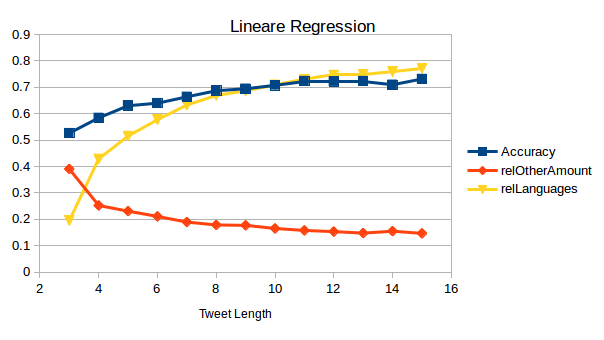
\includegraphics[scale = 0.6]{img/LinearRegressionGraf.png}
\caption{Dependency of accuracy to sentence length together with relative amount of the label "other" and relative amount of the label "lang1" or "lang2" }
\end{center} 
\label{fig:LRSentenceLength}
\end{figure}


\subsection{Accuracy labelling Gibberish}
To take a look at the strengths and weaknesses of the Logistic Regression we labelled 5000 tweets containing 69960 words. We compute the LRs accuracy per label. Our trainingsdata has six different labels. Two of them are actual langauges. Every label is shown in table \ref{tbl:accByLabel}. To compute each labels accuracy we computed the relative amount of correct labelled word for each label:
\[Accuracy_{Label} = \frac{numberOfCorrectLabels}{numberOfLabel}\] 
The results are shown in table \ref{tbl:accByLabel} \\
The table shows that the LR has problems labelling words which are no natural language (other, mixed) and name enteties (ne).  The worst performance has the LR with ambiguous word (Words which are equal in spanish and english e.g. "no") with only 9\%. But only 0.24\% of the labels are ambiguous. Thus is not much improvement for the overall system possible. 
Another good solution shows the LR for \textit{Language Detection}. This is the abbillity to recognise that the word has to be labelled with "english" or "spanish". This could be usefull to brute-force decript cypher texts with unkown keys. The LR can be used to check if the decription includes actual words or is just a failed decription containing only gibberish. The best accuaracy has the LR with english words (87\%). It seems that the bigramms perform really good with english and wors with spanish  (74\%).
\begin{table}[]
\centering
\label{tbl:accByLabel}
\begin{tabular}{ll}
Label& Accuracy \\ \hline
Other     & 0.47 \\
Ne        & 0.44 \\
Mixed     & 0.61 \\
Ambiguous & 0.09 \\
Language Detection & 0.83 \\
Spanish   & 0.74 \\
English   & 0.87 
\end{tabular}
\caption{Accuracy for different labels}
\end{table}


